%%%%%%%%%%%%%%%%%%%%%%%%%%%%%%%%%%%%%%%%%%%%%%%%%%%%%%%%%%%%%%%%%%%%%%%%%%%%%%%%
%2345678901234567890123456789012345678901234567890123456789012345678901234567890
%        1         2         3         4         5         6         7         8

\documentclass[11pt, onecolumn, compsoc, letterpaper]{article}
%\usepackage{times}

% Subfiles package
%\usepackage{subfiles}

% Usual setup packages
\usepackage{listings} % For including source code with highlighting
\usepackage{hyperref} % For better hyper-link integration
\usepackage[bottom]{footmisc} % places footnotes at page bottom

% Packages for verbatim text blocks
\usepackage{alltt} % Package for including math in verbatim text
\usepackage{fancyvrb}

% Packages for math symbols and other mathey things
\usepackage{amsthm}
\usepackage{amsmath}
\usepackage{amsfonts}
\usepackage{amssymb}

% Packages for including pseudo-code
\usepackage{algorithmicx}
\usepackage{algorithm}
\usepackage{algpseudocode}

% Packages that handle tables, figures and other floats
\usepackage{tabularx}
\usepackage{multirow}
\usepackage{float} % To make floats movable
\usepackage{subcaption}
\usepackage[table]{xcolor}

% Packages for drawing graphs, FSMs, etc.
\usepackage{pgf}
\usepackage{tikz}
\usetikzlibrary{shapes,arrows,calc,fit,positioning,shapes.symbols,shapes.callouts,patterns,automata,matrix}

% Remove red boxes around refs
\hypersetup{
    colorlinks,
    citecolor=black,
    filecolor=black,
    linkcolor=black,
    urlcolor=blue
}

% Squeeze whitespace
\usepackage{geometry} % to change the page dimensions
\usepackage[compact]{titlesec}
\usepackage{titling}

\setlength{\parskip}{0pt}
\setlength{\parsep}{0pt}
\setlength{\headsep}{0pt}
\setlength{\topskip}{0pt}
\setlength{\topmargin}{0pt}
\setlength{\topsep}{0pt}
\setlength{\partopsep}{0pt}

\titlespacing{\section}{0pt}{*3}{*3}
\titlespacing{\subsection}{0pt}{*2}{*2}
\titlespacing{\subsubsection}{0pt}{*1}{*1}

\renewcommand{\arraystretch}{1.2}
\setlength{\droptitle}{-2cm}

% ------------------------------ CUSTOM MACROS ------------------------------------
% Nice little macro for adding a comment box. Include incrementing comment numbers.
\newcounter{comcount}
\setcounter{comcount}{0}
\newcommand{\mycomment}[1]
{
\refstepcounter{comcount}
\smallskip\noindent\fbox{\parbox{\linewidth}{\emph{Comment \arabic{comcount}} : \small{#1}}} 
}

% - Math
\DeclareMathOperator*{\argmin}{\arg\!\min\>}
\newcommand{\amin}[1]{\underset{#1}\argmin}
\DeclareMathOperator*{\argmax}{\arg\!\min\>}
\newcommand{\amax}[1]{\underset{#1}\argmax}

\newcommand{\abs}[1]{\lvert#1\rvert}
\newcommand{\norm}[1]{\lVert#1\rVert}
\newcommand{\D}[2][t]{\frac{d#2}{d#1}}
\newcommand{\PD}[2][t]{\frac{\partial #2}{\partial #1}}
\newcommand{\V}[1]{\mathbf{#1}}
\newcommand{\sig}{\mathcal{S}}
\newcommand{\ceil}[1]{\lceil#1\rceil}
\newcommand{\xm}{x_{\hat{m}}}

\begin{document}
\title{Ph.D. Thesis Proposal}
\author{Anshul Kanakia}

\maketitle

\section{Introduction}
The field of swarm intelligence is relatively new one, having become more prominent over the past two decades. As such, it incorporates knowledge from older, well established subjects such as biology (insect colonies and evolutionary biology), mathematics (cellular automata and game theory), robotics (sensor networks and distributed systems), and artificial intelligence (learning algorithms and neural networks). This has led to novel approaches in the design and analysis of multi-agent systems (MAS) and the algorithms associated with them. It has spawned an entirely new field of research called \emph{Swarm Robotics}\cite{Sahin2005}, which has led to a large number of robotic platforms, algorithms, and analyis tools \cite{Brambilla2013}.

Swarm systems have many benefits over traditional, centralized robot systems. The robots used in swarm applications are generally many orders of magnitude smaller (\emph{cm} vs.~\emph{m}, \emph{grams} vs.~\emph{kg}) and simpler in design ($<10$ vs.~$100$s of actuators) than conventional robots, while being much greater in number ($10^2$ to $10^{<<23}$). Also, most swarm systems are homogeneous---robots with identical software/hardware are used to complete the assigned task. This makes swarm systems easily scalable while simultaneously keeping manufacturing and maintenance costs of the hardware low. Though, perhaps their greatest advantage is system stability and robustness to error. Most swarm systems consist of small, relatively simple robots that are only capable of limited and noisy sensing, communication and actuation. This means that while no single robot alone is capable of performing the task assigned, the system as a whole is resilient to individual unit errors and is capable of completing the task \cite{Winfield2005}.

Swarm robotics has tackled a vast array of MAS problems in the past two decades. It's corpus ranges from self-organization, self-assembly, pattern formation, and aggregation to foraging, coordinated movement (such as flocking and schooling), and group surveillance. Performing collaborative tasks is a vast sub-field of study in swarm robotics and a considerable work has been done to understand and model such scenarios, particularly by Ijspeert and Martinoli using the well known stick-pulling experiments. 

Collaborative tasks using MAS extend to a variety of potential real-world applications such as oil-spill containment, firefighting (particularly large forest fires), object transport, and group surveillance and, as such, form an important subclass of problems to study and analyze. Am important question that has so far remained unanswered when attempting collaborative tasks is how many agents are required to complete a given task of a certain size and how are they recruited? It is often assumed that all robots are pre-programmed to form groups of a particular size beforehand or that the task requires an \emph{exact} number of robots to complete successfully---a number that is known beforehand. 

But what about tasks that are dynamic in nature such as fighting forest fires? In such cases it is impractical and often impossible to known beforehand, exactly how many agents are required for successful completion. More importantly, the benefit of increasing the team size of agents for such collaborative tasks increases non-linearly with team size, e.g. Where 1-5 robots may be incapable of lifting a heavy object, 6-7 will be able to lift and move it successfully. I define such tasks with non-linear increase in system utility with increasing team sizes, ``Concurrent Benefit'' tasks. It is for such situations that I propose a novel methodology for estimating group sizes in a distributed fashion, as described by my thesis statement below.

\section{Thesis Statement}
\begin{quote}
My goal is to provide a fully distributed methodology for estimating appropriate team sizes required to complete concurrent benefit tasks using a multi-agent system. I will analyze this methodology using tools from various disciplines to provide theorems on overall efficiency and resultant group behavior while supporting these claims using numerical and physics-based simulations as well as real robot experiments using the \emph{Droplet} Swarm Robot platform.
\end{quote}

This approach to solving the problem of group size estimation differs from existing approaches in swarm robotics that are often constrained by the inherent physical and memory limitations of small, simplistic robots. Applications of MAS to real-world scenarios is lacking today because many of the existing swarm robot platforms are exceedingly simplistic and are not capable of handling complex tasks such as rough terrain traversal, carrying heavy objects, long-distance communication, etc. that are required for tackling actual situations. While the focus of my research is not on hardware design (far from it!), I aspire to develop a more adaptable and mathematically rigorous solution for group size estimation and recruitment that is oblivious to the physical restrictions of a robotic platform and works in almost all MAS settings. The only assumptions I make reasonably are that whatever hardware my algorithms run on is capable (however imperfectly) of the four basic requirements of robotics; actuation, sensing, communication and computation.

\section{Proposed Work}
In this section I will outline my proposed research work, focusing heavily on two main aspects of my thesis statement; modeling and analysis of swarm systems and my specific work on team size estimation, in that order.

\subsection{Consistent Modeling Methodology for Swarm Robotics}
The first issue any swarm robotics researcher faces is a distinct lack of established modeling methodology in the field.  This is why review papers is swarm robotics as recent as 2007 \cite{Bayindir2007} still cite modeling as an open research topic for the field. While a number of disconnected methods exist for modeling large swarms, there is currently no unified way of going from actual physical hardware experiments to simulations and models and back. 

In order to make swarms an alternative engineering approach---in which robustness emerges despite predictable, individual failure---we require formal tools that allow us to predict and verify the resulting complex behavior. Developing such tools goes hand-in-hand with investigating novel hardware (Figure \ref{fig:swarmbots}), simulation tools \cite{Michel1998}, and tracking tools \cite{correlliros06,lochmatter08} that ease conducting large numbers of experiments with large numbers of robots. Analyzing swarm dynamics on a higher abstraction level allows us to explore the design space much faster, but also to use parameter analysis and numerical methods for optimization and verification.

\begin{figure}
	\centering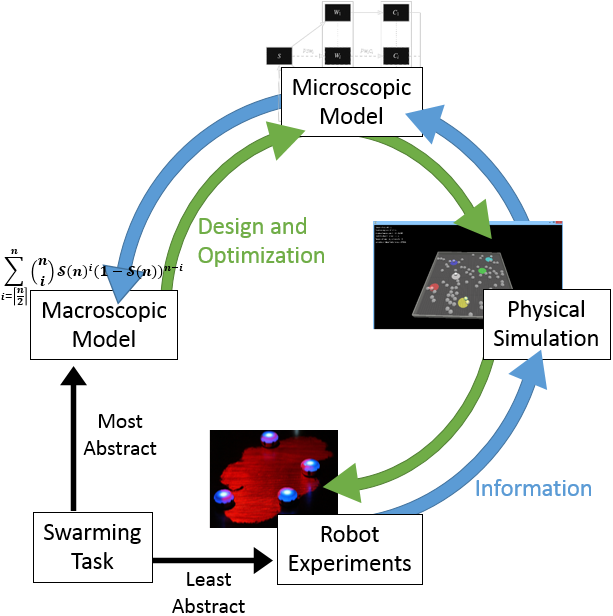
\includegraphics[width=.75\textwidth]{../assets/ssmodel.png}
	\centering\caption{}\label{fig:ssmodel}
\end{figure}

For this purpose, I propose a closed loop system as seen in Fig.~\ref{fig:ssmodel}. Setting up the required swarming task as a real physical experiment or physical simulation allows us to discover and measure the different free parameters in the system. We then use these variables in lower resolution models (micro-level) as well as in the development of mathematical models (macro-level) for our system. These more abstract models allow us to rapidly experiment with system parameters and optimize them. We can then use these optimized parameters back in the real physical experiments to improve the desired behavior of the system and repeat the cycle till the desired level of accuracy and satisfaction of model behavior is achieved. A closed loop modeling methodology also allows us to identify and optimize important system parameters as described in \cite{Correll2006a,Correll2008}.

\subsubsection{A Spatial Modeling Paradigm for Swarm Robotics}
Perhaps the simplest way to model a physical system is to write out the equations of motion associated with each individual agent in the system. This approach has been applied in some cases such as animal herding\cite{Correll2008b} where a relatively small number of agents are involved. 

As one can imagine though, modeling every single micro-level interaction between agents quickly gets out-of-hand for very large systems, being analogous in complexity to the n-body problem in physics. The complications that arise when trying to understand these multi-object systems are thus non-trivial, but all is not lost! The established discipline of statistical physics has been tackling these very issues for decades now. Well understood strategies and tools exist for extracting macro-level properties from systems with micro-level particles numbered in the order of Avogadro's constant, $10^{26}$.

We can leverage these tools from statistical physics for understanding and modeling swarm systems as well, even though the number of agents we typically deal with are many orders of magnitude smaller. The use of spatial modeling for swarm robotics has become increasingly popular in the past few years, as is evident from the work of Hamann\cite{Hamann2008, Hamann2010}, Prorok et al.\cite{Prorok2011}, Milutinovi\`{c} and Lima in\cite{Milutinovi2006}.

The central strategy used in spatial modeling of swarm systems involves the use of the Langevin equation, originally used for describing the Brownian motion of a large particle suspended in a medium of smaller particles, e.g. A pollen grain in oil. The Langevin equation is defined as follows\cite{Reif1965}.
\begin{equation}
	m \frac{d\dot{x}}{dt} = \mathcal{F} + F' - \alpha\dot{x}
\end{equation}
Where $\mathcal{F}$ are the forces exerted on the particle at a macroscopic level, $F'$ are the small micro-level fluctuations whose ensemble average $\left<F'\right> = 0$. The final negative term $\alpha\dot{x}$ accounts for friction forces or viscous drag experienced by the large particle during motion. It is important to note that the Langevin equation is any differential equation that describes the temporal and spatial evolution of a subset of the degrees of freedom of a particle, i.e. it is not a single equation but a class of equations that all describe the same phenomenon. 

\begin{figure}[!htb]
\centering\begin{subfigure}{.5\textwidth}
\centering\includegraphics[width=7cm]{../assets/LanNoDrift.png}
\end{subfigure}~
\centering\begin{subfigure}{.5\textwidth}
\centering\includegraphics[width=7cm]{../assets/LanDrift.png}
\end{subfigure}
\caption{Left: Solution to Langevin equation for a particle in 1D with $\V{A} = 0$, i.e. no drift. Right: Solution with $\V{A} = 0.1$. In both cases the diffusion coefficient is constant, $B = 0.3$, and $\V{F}$ uses an uncorrelated normal distribution with mean $\left<\V{F}\right> = 0$.}\label{fig:lan}
\end{figure}

From the Langevin equation above, we can derive the macro-level Fokker-Planck equation as stated below,
\begin{equation}
\PD{\rho(\V{r},t)} = -\nabla(\V{A}(\V{r},t)\rho(\V{r},t))+\frac{1}{2}Q\nabla^2(B^2(\V{r},t)\rho(\V{r},t))
\end{equation}
\begin{figure}[!ht]
\centering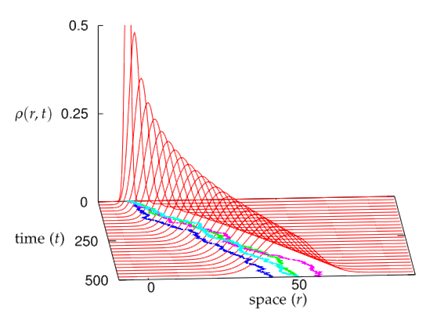
\includegraphics[width=7cm]{../assets/fokkerPlanck.png}
\centering\caption{A visual comparison between the spatial micro vs. macro-level equations. The colored lines on the $r$-$t$ plane show the paths taken by individual particles, found via the Langevin equation, while the overarching red curve is the probability distribution for the entire ensemble as described by the Fokker-Planck equation.}\label{fig:fokkerplanck}
\end{figure}

A clear and concise derivation of the above equation from the Langevin equation is provided in section 4.1 of \cite{Hamann2010}, which in turn follows closely from the book \emph{Synergetics} by Haken (1977). The terms $\V{A}$, $B$ and $\V{F}$ reprise their earlier roles from the Langevin equation, while $Q$ is a new displacement term due to collisions between particles. $\rho(\V{r}, t)$ is the probability of encountering a particle at position $\V{r}$ and time $t$. As one can see, the Fokker-Planck equation gives us a \emph{probability distribution} of the positions of particles in space, making it a viable macroscopic model compared to the micro-level Langevin equation which gives us the \emph{position} of a \emph{single} particle in space (see Figure~\ref{fig:fokkerplanck}).

The Fokker Planck equation is a relatively new tool in the field of swarm robot modeling and has notably been used by Hamann\cite{Hamann2008,Hamann2010}, as well as Prorok, Correll and Martinoli\cite{Prorok2011} in their work on boundary coverage and inspection of jet-turbine engines using swarms of miniature robots. They used a hybrid approach for modeling collective inspection that involves a probabilistic non-spatial model coupled with spatial micro-macro diffusion equations for modeling collective inspection of regular structures to improve consensus with observed experimental values. 

\begin{figure}[!htb]
\centering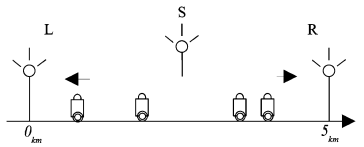
\includegraphics[width=.75\textwidth]{../assets/spatSignal.png}
\centering\caption{Experiment setup for centralized robot population control experiment proposed by Milutinovi\`{c} and Lima in%\cite{Milutinovi2006}
.}\label{fig:signal}
\end{figure}

A spatial model also is used in\cite{Milutinovi2006} to control a large scale multi-agent system using centralized controller and three signal sources. A visual representation of this setup can be seen in Figure~\ref{fig:signal}.

\subsubsection{\emph{Droplet} Hardware and Simulation Platform}
An important step in any modeling process is validation by comparing model results to real experiment data. Given the relatively abstract approach we have seen so far for designing models of robot swarms, this step is made even more crucial. The micro and macro-models in swarm robotics have conventionally been designed using observed phenomena from other processes seen in biological and chemical systems and adapted to fit the swarming task being studied. Many swarm algorithms show emergent behavior where the observation of complex properties at the system level cannot be trivially inferred from studying the individual agent behavior. The generalizations and simplifications made in the robot controller design when developing the micro and macro-models can, and in many cases do, suppress the interesting emergent properties seen in real physical systems. 

To be able to accurately recreate a task on a swarm system without investing the substantial time and resources required to develop and deploy real robots, we use physics-based simulators. The point of these simulators is to remain as true to the real world as possible while maintaining an order of magnitude improvement in speed and simplicity over real robot experiments. Unlike micro-models that abstract away physical and environmental issues such as wheel slip, sensor noise, communication delays, etc., using probability and dice rolls, physics-based simulators make the added effort to accurately and dynamically model every minute aspect of the swarm system.

\begin{figure}[!htb]
\centering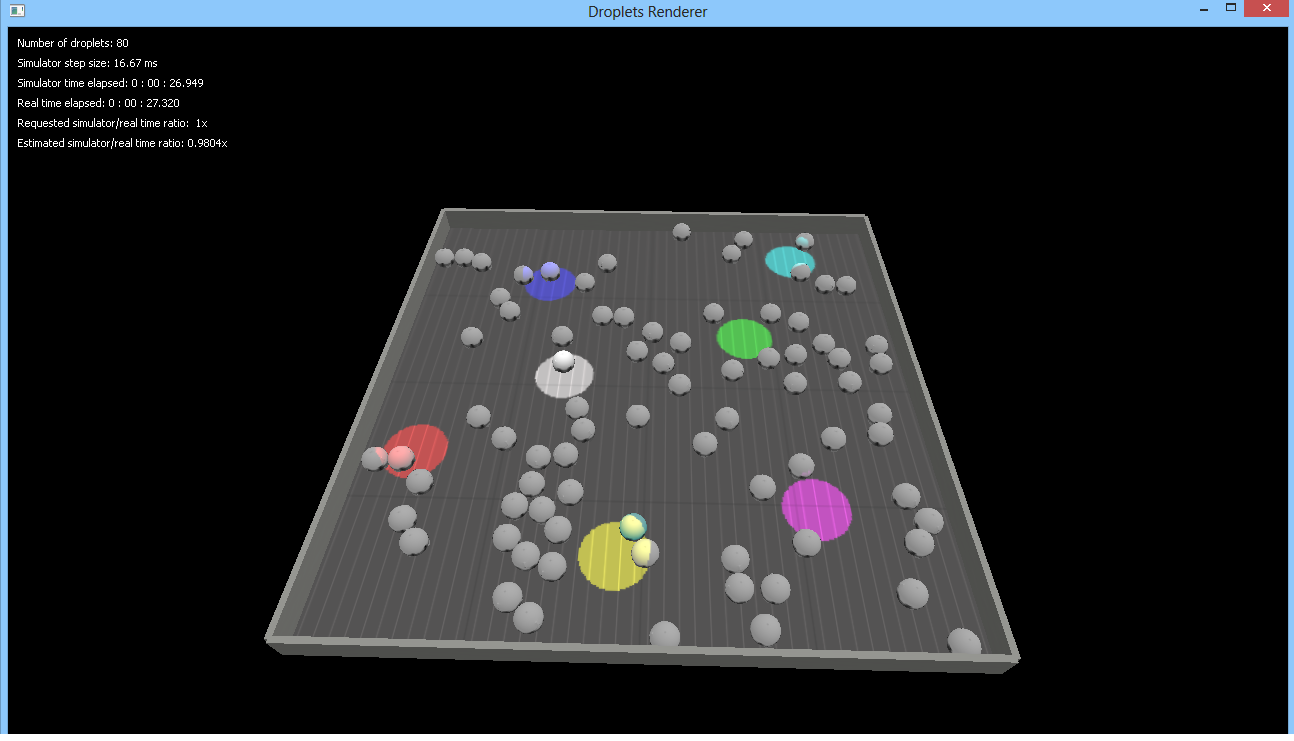
\includegraphics[width=.75\textwidth]{../assets/dsim.png}
\centering\caption{The Droplet swarm robot simulator}\label{fig:dropletsim}
\end{figure}


\subsection{Collaboration Model using a Sigmoid Threshold Function}
I have already studied how sigmoid threshold functions can be used as a voting mechanism in collaboration problems for determining sufficient team size. We can tune the logistic function, as seen below, using two parameters $\tau$ and $\theta$ which map to the mean and variance for desired team sizes, respectively.

\begin{equation}
	\sig(\xm) = \frac{1}{1 + e^{\theta(\tau - x)}}
\end{equation}


\subsection{Application of Game Theory to MAS}
One such tool that is becoming increasingly applicable to the field of swarm robotics is \emph{Game Theory}. Being formally introduced in John von Neumann's seminal work, "Zur Theorie der Gesellschaftsspiele" (On Theory of Games and Strategy) in 1928, game theory has since been applied to a vast array of fields such as economics, biology and, more recently, computer science to study the mathematical models of conflict and cooperation between intelligent rational decision-makers.

\subsubsection{Global Games}



\section{Conclusion}

% Bibliography
%\nocite{*} % Show all Bib-entries
%\bibliographystyle{plainnatCustom}
\bibliographystyle{plainCustom}
\bibliography{../refworks}

\end{document}